\documentclass[12pt,a4paper]{article}

\usepackage{ucs}
\usepackage[latin1,utf8x]{inputenc}
\usepackage{amsmath}
\usepackage{caption}
\usepackage{subcaption}
\captionsetup{font=small,labelfont=bf}
\usepackage{listings}
\usepackage[british,english]{babel}
\usepackage{amsfonts}
\usepackage{amssymb}
\usepackage{enumitem} 
\usepackage{graphicx}
\usepackage[lmargin=2cm,rmargin=2cm,tmargin=3.3cm]{geometry}
\usepackage{subfiles}
\usepackage[final]{pdfpages}

\setlength{\parindent}{0pt}
\setlength{\parskip}{1ex plus 0.5ex minus 0.2ex}

%insert links
\usepackage{hyperref}
\usepackage{xcolor}
\definecolor{dark-red}{rgb}{0.4,0.15,0.15}
\definecolor{dark-blue}{rgb}{0.15,0.15,0.4}
\definecolor{medium-blue}{rgb}{0,0,0.5}
\hypersetup{
    colorlinks, linkcolor={dark-red},
    citecolor={dark-blue}, urlcolor={medium-blue}
}

%
\usepackage{float}
%\restylefloat{figure}

\usepackage{fancyhdr,lastpage}	
\pagestyle{fancy}

%header
\lhead{ 
	SANS Holiday Hack Challenge \\
}
\chead{ 
}
\rhead{ 2016 \\  }

%Footer
\lfoot{
	\rule{\textwidth}{0.1mm}\\
}

\cfoot{}
\rfoot{\ \\ \scriptsize{Page \thepage\ of \pageref{LastPage}}}

\begin{document}

%Forside
\begin{titlepage}
	\begin{center}
		\vspace*{13\baselineskip}
		\huge
		\bfseries
		SANS Holiday Hack Challenge 2016\\ 
		\ \\
		Write-up \\[5\baselineskip]

		\small
		\vfill
	\end{center}	
	\begin{flushleft}
		By Regenuluz\\
		\ \\
	\end{flushleft}
\end{titlepage}

\ \\
\section*{Introduction}
\label{section.intro}
	SANS Holiday Hack Challenge.\\
	\\
	This is the first time I participate in it and it is also the first ever write-up I've done of any CTF, so this should be fun.\\
	\\
	Also, a chance of winning a t-shirt, no matter how much one manage to solve? Count me in, I love free t-shirts, seriously.\\
	\\
	Now really, this is more than enough of an introduction, this write-up is running late as-is. I've probably spend more time actually converting my text document with my solutions into something that can be shared and understood by anyone other than me. Check \autoref{app.notes} for the original notes.

\thispagestyle{empty} 
\newpage

%Table of Contents
\thispagestyle{empty} 
\tableofcontents
\thispagestyle{empty} 
\newpage

%Reset pagecount
\setcounter{page}{1}

%Alm. sider
\ \\
	
\subfile{part1.tex}
%\newpage
\subfile{part2.tex}
%\newpage
\subfile{part3.tex}
%\newpage
\subfile{part4.tex}
%\newpage
\subfile{part5.tex}
%\newpage

% Quests
\subfile{quests.tex}
\newpage

\newpage
\appendix
\section{The mad notes} \label{app.notes}
	For the curious people, here's how the notes that I took during this challenge looks. I didn't take notes of the Netwars coins for the first 5-6 coins or so, so for this write-up, I had to go back and locate them all, again, to get my screenshots. Well, enjoy.
	
	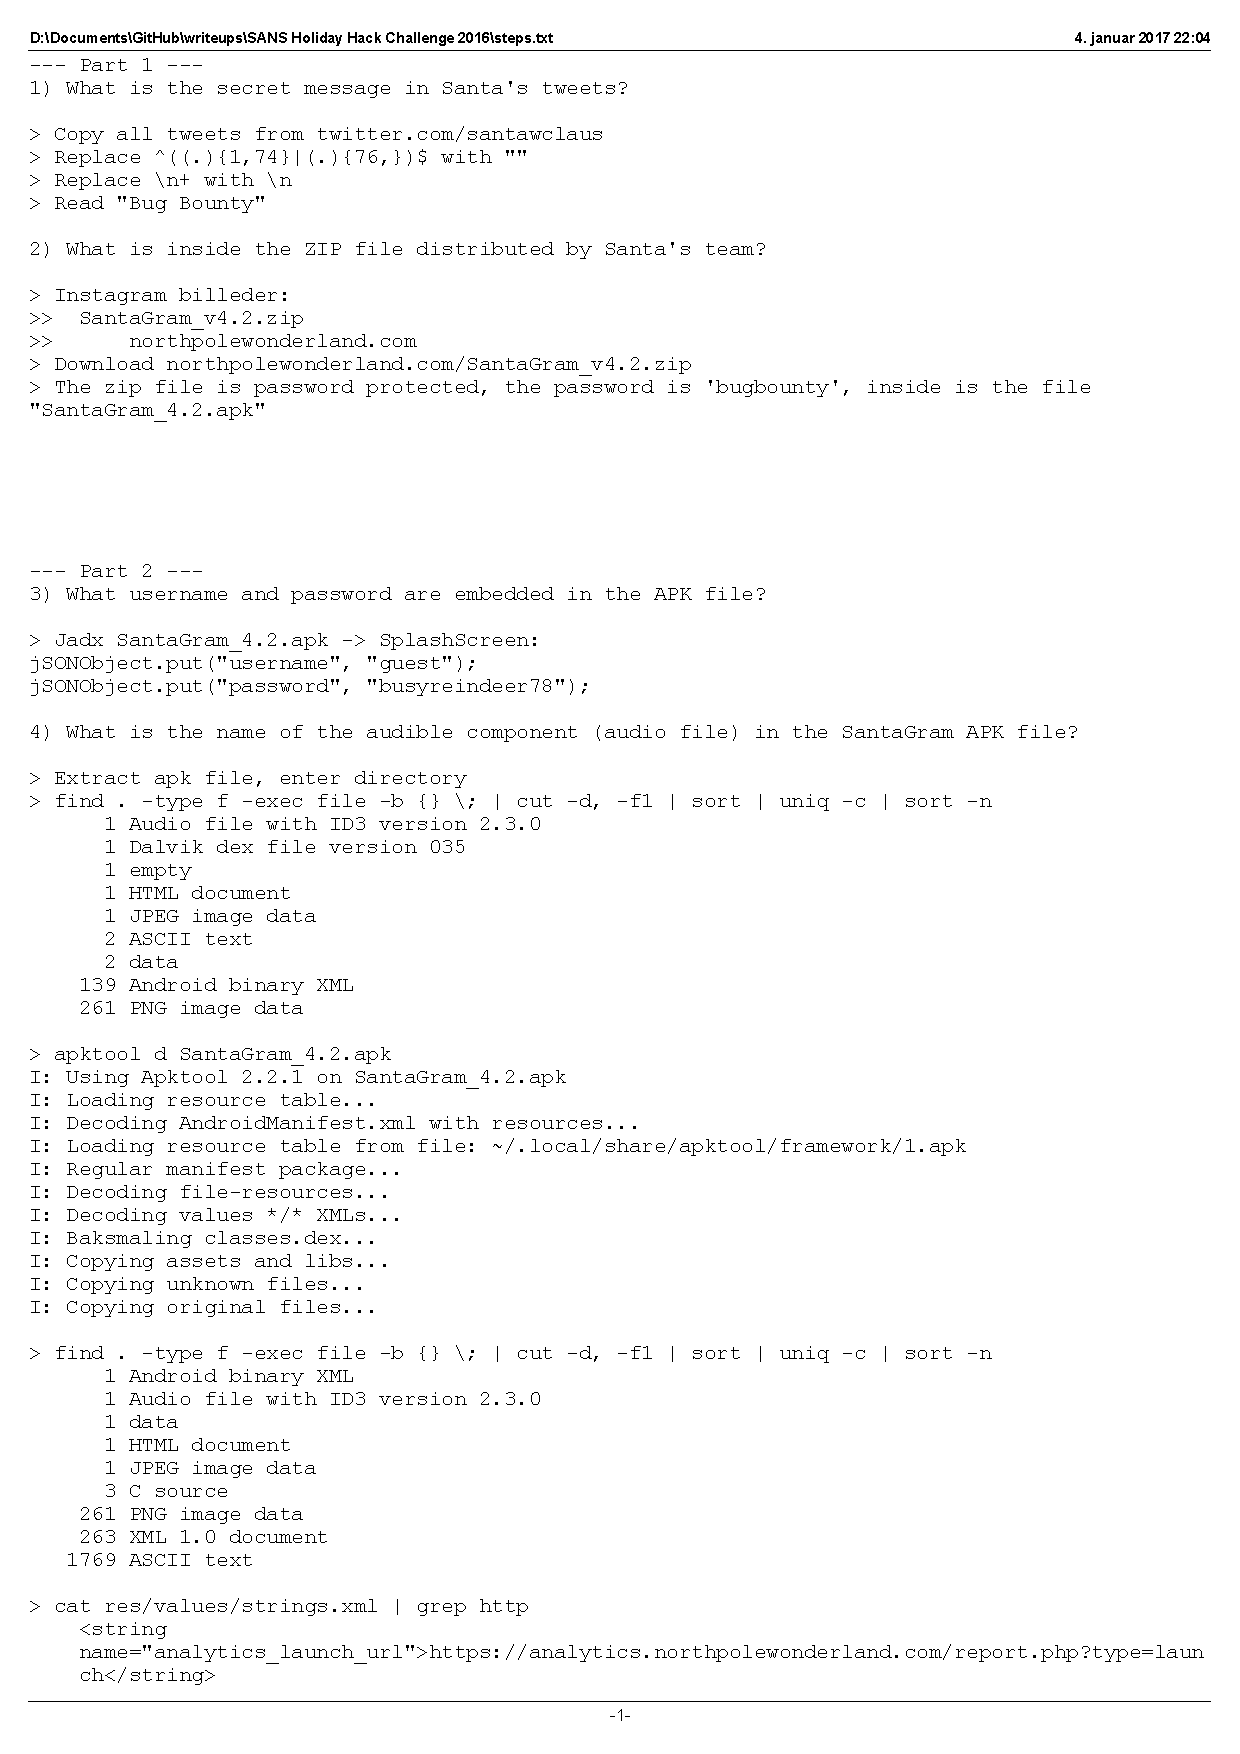
\includepdf[pages=-,width=\textwidth]{steps.pdf}

\end{document}